\chapter{Software-defined Storage Systems: Design and Implementation}
\label{chap:syndicate_sds}

In order to validate the design principles of software-defined storage, this 
thesis presents the design and implementation of two separate SDS systems.
Both systems currently enjoy use in production environments.
The first system, called Gaia, implements a global key/value store with programmable semantics for its
\texttt{get} and \texttt{put} operations.  It is a minimalistic SDS system---it
provides just enough functionality to ensure that applications and
users can interact with their under a fixed set of storage
semantics running at a layer above the third-party services.

The second system, called Syndicate, implements
a full POSIX filesystem interface with programmable semantics for most
filesystem operations.  It is much more featureful than Gaia, and is designed
to port existing scientific computing workloads to commodity third-party
services.

Despite being designed for different use-cases, both Syndicate and Gaia allow
developers to preserve end-to-end storage semantics while respecting
organizational autonomy.  Both systems achieve this by providing one or more
gateway implementations that run in separate organizations, but
coordinate through a shared untrusted metadata service.  While the systems have
different gateway and MS designs and implementations, they nevertheless adhere to
the same design principles.

\section{Gaia: a Global Key/Value SDS System}

Gaia is a global key/value store designed for users to host their data
for decentralized Web applications.  In this thesis, ``decentralized''
applications are applications where all of the business logic runs on the
users' computers.  For example, a decentralized todo-list
application~\cite{blockstack-todo} would fetch the user's application state from
the storage providers of their choice, allow the user to interact with the items
once loaded, and would store the resulting state back to the storage providers
when the user is done.  Unlike conventional Web applications,
there is no ``application server'' that runs business logic on the user's data.

Gaia is designed for Web programming environments, and offers two
modes of operation.  The first mode, called ``single-reader mode,'' offers
behavior similar to what Web developers today expect from HTML5
\texttt{localStorage}~\cite{w3c-localstorage}.  The Web code can load a value
given a key and store a (key, value) pair, with the expectation that only this
instance of the code will be able to interact with the key.  For example, 
the aforementioned to-do list application would use this mode to ensure that a user can
only read and write their own data, and other users cannot interact with it at
all.

The second mode, called ``multi-reader mode,'' offers one-writer many-readers
semantics.  Only a user may write to their own keys, but any user may discover
and read their keys.  For example, a blogging application built on Gaia would
use Gaia's multi-reader mode to allow a user to publish blog posts, and allow
other users to read them.

The main contribution of Gaia is to give Web developers a secure and
reliable way to outsource data-hosting to users.  Gaia ensures that each user
securely and automatically discovers each other users' volumes and certificate
graphs for each application they use prior to loading the data.
In doing so, Gaia offers end-to-end
data authenticity and confidentiality while using untrusted commodity cloud infrastructure
to host and serve application data.

Despite being a minimalistic SDS system with a simple API, it is used today on
production workloads for Blockstack~\cite{blockstack} applications.  Many
non-trivial applications rely on it for storage, including a shared document
editor~\cite{graphite-docs}, a cryptocurrency portfolio
manager~\cite{coins}, a microblogging
platform~\cite{publik}, and
an end-to-end encrypted Web chat application~\cite{stealthy.im}.

\subsection{Motivation}

In conventional Web applications, users and would-be developers are severely
constrained in what they are able to do with their data.  This is because in
conventional Web applications, the business logic and the storage logic both run
in the application's servers.  As such, all authoritative replicas are hosted
outside of the users' organizations, and any computations that may be performed
over them are mediated by the application's servers.  Users and would-be
developers need \emph{permission} to access, modify, and extend their data's
storage.

The motivation for creating Gaia is to allow Web applications to be written in a
way that decouples business logic from storage logic.  Users and developers
ought to be able to control where their data is hosted and how reads and writes
on it are carried out.  At the same time, making this change should not require
Web application developers to significantly re-think the way they build
applications---at most, they should only have to change the Javascript calls in
their application frontends to direct reads and writes to the users' chosen
storage providers, instead of the application servers.  Achieving this would
yield three main benefits:  (1) users can keep their data in the
event that its developer stops maintaining the application, (2) multiple
applications can interoperate by reading from each other's volumes, and
(3) developers can avoid the need to host user data, or any ``hard state'' for
their applications.

These benefits are realized by first observing that in many cases,
a Web application's data interaction model is \emph{already} centered around
individual user activity.  Users can read and write their own data, but can
only read other users' data.
In applications that present ``shared-write'' views of data, like a comment section on a blog or
a shared Google Document page~\cite{google-docs}, the business logic
attributes each write to a specific user, and then ``merges'' their
writes to present a consistent view.  Gaia exploits this property of Web
applications by bundling up all of a user's data into its own volume, and giving
the volume owner the ability to grant other users read access to it.

\begin{figure}[h]
   \caption{Gaia versus traditional Web applications.  In traditional Web
   applications (left), application clients' reads and writes are mediated
   through a shared application server.  In Gaia, reads and writes are processed
   by a sequence of one or more Gaia nodes before being loaded and stored to
   commodity storage as chunks.  Gaia nodes, in turn, run the users' gateways.}
   \centering
   \includegraphics[width=0.9\textwidth,page=16]{figures/dissertation-figures}
   \label{fig:chap3-gaia-vs-traditional-web}
\end{figure}

Even though a Web application has a single logical database that holds all of
its users state, this observation about access patterns allows Gaia to reformulate
the global database as a collection of single-writer multi-reader user-specific
databases (Figure~\ref{fig:chap3-gaia-vs-traditional-web}).
It becomes the application client's job to translate a set of reads across
the users' databases into a consistent view, whereas this had traditionally been
done by the application's global database.  In SDS terms, both the
Web applications and each users' computers form separate organizations, and each
organization sets a policy that allows writes only from within the organization
and allows reads from zero or more other organizations.

This reformulation of application storage gives Gaia the ability to separate each
users' piece of the Web application's global state into its own volume, thereby
placing it under the control of the user's organization.
The application only needs to be able to read from a user's database piece in order to
present other users with a view of its data.  The database need not reside on
servers that the application developer chooses.  What this means in SDS terms is
that there is one volume per $(application,user)$ pair, and that only the user may
write to the volume and control its access semantics.  Application developers
are simply considered users of their own application.

A user may optionally make a volume readable to another set of users, or to the
world.  For example, users of a blogging application would make their volumes
world-readable.  As another example, the application developer's volume would
store application assets like images, CSS, and code to be loaded at runtime by
the running application code (thereby allowing the developer to push
updates to their application, much like how they do today on the Web).

The SDS design principles come into play in the following tasks:

\begin{itemize}
   \item \textbf{Multiple Storage Systems}.  Gaia allows users
      to choose the storage systems that will host their data in an
      application-agnostic way.
   \item \textbf{User Storage Policies}.  Gaia allows users to
      stipulate programmatic policies pertaining to data availability and
      durability, thereby preserving organizational autonomy.
   \item \textbf{Application-specific Views}.  Gaia uses aggregation
      drivers to construct global, consistent views of a set of users'
      application state, thereby preserving end-to-end storage semantics.
\end{itemize}

\subsection{Blocks, Manifests, and Volumes}

Gaia organizes a user's data into a set of volumes, where each volume
holds one application's data.  The user decides whether or not the volume
operates in single-reader or multi-reader mode, and selects the set of
service drivers to use to replicate data.

A volume in Gaia is a key/value store.  The API the Gaia client exposes to
programmers resembles HTML5's \texttt{localStorage}.  It offers three methods:
\texttt{get(key): value}, \texttt{put(key, value): bool}, and
\texttt{delete(key): bool}.  The writers to the volume are the gateways that run
on the user's trusted devices.  The readers are either exclusively the user's
devices (in the single-reader mode), or any device that can discover the
publicly-visible data (in multi-reader mode).

Internally, the set of keys in a volume are bundled into a per-device manifest.
Each value is the associated block, which points to replicas of the raw data.
This means that per-device writes are serialized
across keys, and that writes to a key are atomic.  These behaviors were chosen
specifically to emulate the semantics of \texttt{localStorage}.

\subsection{Gateways}

Users run one or more Gaia nodes to access their application state.  Gaia nodes,
in turn, run gateways on behalf of the application.  The Gaia node the
application accesses provides a key/value storage abstraction that encompasses
all of the key/value pairs written by all of the user's devices.  It forwards
reads and writes to gateways running within this and other Gaia nodes.

Gateways in Gaia are realized partially-evaluated code within the Gaia
node.  Instantiating a gateway is cheap---the node simply allocates
a new internal \texttt{gateway} object and pairs it with an
application-specific context.

Gateway instantiation and teardown is driven by application sign-ins.
When the user signs into the application, the Gaia node instantiates gateways to
run access and mutate flows.  When the application's Web page writes data,
it asks the user's Gaia node to run a mutate flow through its Build, Push, and
Publish gateways to make the write durable and avaialble.
Each of the user's devices runs a Gaia node locally or on a trusted host to
process writes.  The device running the node with the writing gateways
must be trusted, since it runs coordinator gateways and has access to their
private keys.

The read path depends on whether or not the volume is a single-reader or
multi-reader volume.  If it is a single-reader volume, then the Web page simply
asks the user's own Gaia node to carry out the access flows.  If it is a
multi-reader volume, then the Web page instead contacts the Gaia metadata
service (discussed below) to find the Gaia node that can serve the data.
Once this node is known, the Web page asks the node to
carry out the access flow.

Because a user may have multiple devices, there can be multiple writers to
a single volume.  Gaia assumes that \emph{application writes are
sequentially consistent}.  This is a reasonable assumption in practice, because
(1) a volume may only be written to by the user
that owns it, (2) a user typically does not access the same application from
two different devices simultaneously, and (3) any concurrent writes from the
application on the same device can be serialized by the Gaia node.

\begin{figure}[h]
   \caption{Application interface to Gaia.  Gaia combines the timestamped
   key/value writes in each device's manifest to create a coherent view of the
   user's volume.}
   \centering
   \includegraphics[width=0.9\textwidth,page=17]{figures/dissertation-figures}
   \label{fig:chap3-gaia-global-key-value-store}
\end{figure}

This assumption side-steps the need for a user's Gaia nodes to
coordinate to resolve write-conflicts in the key/value abstraction.  Since each
device runs the coordinator gateway for the key/value pairs it has
written, the key/value abstraction can be realized simply by
merging each device's key/value pairs into a single key/value space.
The merge function simply accepts the
value with latest timestamp in order to handle cross-device
key/value conflicts (Figure~\ref{fig:chap3-gaia-global-key-value-store}).

In the rare cases where an application expects a user to read and write from
multiple devices simultaneously, the developer has the opportunity to implement
write serialization in the volume's aggregation driver.  The absence of built-in
write/write conflict resolution is a design choice that makes the common case
simple in its implemetation and performant in its execution. 

\subsection{Metadata Service}

Gaia nodes implement a peer-to-peer metadata service.  The Gaia MS is based on prior work
on Blockstack~\cite{blockstack}~\cite{virtualchain}~\cite{ali2017}.  It enables
Gaia nodes to both ensure that readers do not see stale data, and to ensure that
any Gaia node can discover and read key/value pairs from a given volume for any user.

Gaia uses a blockchain-based SSI system both for bootstrapping trust between
users and for implementing the ``volume discovery'' and ``gateway discovery''
functions of its MS.  When users Alice and Bob 
register their user names in the SSI, they each include a cryptographic hash within the
blockchain transaction.  This hash corresponds to a DNS zone
file~\cite{rfc-zone-file} that contains routing information for discovering the
user's volumes and Gaia nodes.

Gaia nodes work with the SSI system to build a 100\% replica of all zone files.
They self-organize into an unstructured
peer-to-peer network through which they exchange zone files.  They exchange
bit-vectors with one another to announce the availability of their zone files,
based on the sequence of transactions the SSI system has processed that include
new zone files hashes.  Peers inspect one another's bit-vectors, and pull
zone files from one another in rarest-first order such that they all eventually
build a 100\% replica.

Peers arrange themselves into a K-regular peer graph.  They each choose an
unbiased random sampling of the peer graph as their neighbors using a
Metropolis-Hastings random graph walk with delayed acceptance~\cite{lee-xu-eun}.
The default implementation chooses $K=80$, and when queried for neighbors, will
respond with a random sample of at most 10 peers that
have historically responded to queries at least 50\% of the time.  This helps
each peer quickly discover ``healthy'' peers in its neighbor set.  In addition,
each peer remembers and periodically pings up to 65536 discovered
peers regardless of their perceived health in order to accomodate churn in both
the set of peers as well as the network links between them.  For example, a
healthy peer that goes offline for a time due to a bad network link or
misconfiguration will not be completely forgotten for some time, giving the
operator a chance to correct the issue and quickly rejoin the network.

Since Gaia nodes view the same blockchain, they calculate the same sequence of zone
file hashes.  This gives them a ``zone file whitelist'' that grows at a constant
rate, no faster than the blockchain.  They use the whitelist to identify only
legitimate zone files, and rely on the blockchain to ensure that not too many
new zone files can be introduced into the system at once.  A detailed
description of the peer network can be found in~\cite{ali2017}.

\begin{figure}[h]
   \caption{Volume lookups in Gaia.  When Alice wants to read Bob's app data, she
   (1) looks up his ID in his SSI database, (2) finds his zone file in
   Gaia's peer network, (3) finds his certificate graphs, (4) finds his
   public-facing Gaia node and volumes, and (5) routes access flows through it
   to access his volume data.}
   \centering
   \includegraphics[width=0.9\textwidth,page=18]{figures/dissertation-figures}
   \label{fig:chap3-gaia-volume-lookups}
\end{figure}

The peer network ensures that each Gaia node knows the names, current public
keys and current zone file for each user.  Each user's
zone file points to a set of signed volume and gateway configuration data
structures, including the certificate graphs for each volume. 
This way, a Gaia node can
look up an application-specific volume for a user given the user's name on the
SSI system (Figure~\ref{fig:chap3-gaia-volume-lookups}).  Importantly, the networks and storage
providers hosting zone files and configuration data are \emph{not} part
of the trusted computing base.  As long as the user's local SSI server is
trusted, then they can discover authoritative state about other users' volumes.

Discovering a user's data is a matter of first looking up the volume metadata, and then
searching the key space in the metadata for the desired metadata record.  After
Discovery, the reader caches the key's version number, so subsequent reads do
not return stale data.  Publishing data is a matter of uploading a new key/value
pair with a greater version number.

\subsection{Aggregation Drivers}

Users enforce end-to-end storage semantics for multi-reader volumes by standing up and running
publicly-routable Gaia nodes to process reads from other users
(Figure~\ref{fig:chap3-gaia-reads-writes}).  By design,
these public read nodes are \emph{not} trusted, and the gateways they run do not
have any write or coordination capabilities.  The data they serve is
meant for external consumption.

\begin{figure}[h]
   \caption{Gaia read/write configurations.  Discover and Acquire happen in the
   same node in single-reader configurations, but can happen either on untrusted
   nodes or on both trusted and untrusted nodes in multi-reader settings.
   Mutate flow stages always run within the trusted computing base, however.}
   \centering
   \includegraphics[width=0.9\textwidth,page=19]{figures/dissertation-figures}
   \label{fig:chap3-gaia-reads-writes}
\end{figure}

When a user Alice creates a volume, she simply lists the Gaia node
in her signed Gaia configuration as the ``read'' endpoint.  When others Bob and Charlie go to
read from her volume, their Gaia nodes issue the request to her ``read'' Gaia node
indicated by her configuration data.  Bob and Charlie discover the ``read'' node 
by querying the MS.

\subsection{Flow Routing}

Only Alice can change her volume and node configuration.  She does so simply by
regenerating the configuration and signing it with the key listed under her
account in the SSI system.  If she wants to change the URLs to her signed
configuration, she uploads her configurations to the new locations, generates a
new zone file with URLs that point to them, and announces the new zone file's
hash in the SSI system's blockchain.  Once the SSI system processes the
transaction, she broadcasts the new zone file to Gaia's peer network so all
other Gaia nodes can discover her volumes.

When Bob wants to read Alice's data, his node first inspects her volume record
to determine the ``read'' endpoint.  When Bob's node runs the Discover and
Acquire stages, the ``read'' endpoint is given to the aggregation driver as part
of its execution context so it can pull data from it.

When Alice wants to write to data to a volume, her Gaia node ensures that the
appropriate gateways are instantiated with the Build, Push, and Publish stages
from her configuration.  Once they are available, the node processes her write
request.  In practice, her gateways are locally available for the duration of an
application session---her node instantiates them as part of an application
``sign-in'' process, and shuts them down when the session ends.

\subsection{Administration}

To minimize coordination between developers and users, Gaia
automates as much of the system administration as possible.
In its day-to-day operation, the only administrative contact a user has with their volumes is
in connecting storage providers, which is handled via a provider-specific Web
UI.  In addition, Gaia minimizes the instances where the user directly interacts with cryptographic keys
by ensuring that they only need to do so when they acquire or lose a personal
computing device.

Application developers do not interface directly with storage providers, but
instead with the user's designiated Gaia node.
Instead, developers specify the storage requirements the
application needs, and the Gaia node pairs the requirements with storage drivers
when creating its volume.
%A table of storage requirements can be found in
%Table~\ref{tab:gaia-storage-requirements}.

% TODO: table of Gaia storage classes

The application code discovers a user's Gaia node as part of the SSI sign-in
process.  The SSI service identifies to the application the network address
of the user's Gaia node.  The application then learns the set of Gaia storage
providers, and the set of capabilities they offer (which can be matched to
storage requirements).

The resulting storage administration workflow for users and developers works as
follows:

\begin{itemize}
   \item When the user creates an account in the SSI service, she connects one
      or more storage providers to her account.
   \item The user loads the application and clicks its "sign-in" UI element.
   \item The application redirects the user to the SSI service's "sign-in" UI,
      which prompts the user to authorize the sign-in request.  Specifically,
      the user is presented with the application's request for either a
      ``single-reader'' or ``multi-reader'' volume.
   \item Once approved, the SSI service redirects the user back to the
      application, passing it a session token which identifies the user's Gaia
      node.
   \item The application requests a volume.  If this is the first such request,
      the Gaia node creates an application-specific volume.  The node then
      returns a handle to the volume which the application subsequently uses to
      load, store, and delete keys.
\end{itemize}

At no point are users asked to interact with volume, user, or gateway keys, and at no point
are users asked to perform access controls.  At no point are the developers
asked to identify or bootstrap a connection to storage providers, and at no
point are developers required to perform any access controls beyond deciding
whether or not their app-specific volume will be world-readable or private
(enforced internally through encryption).  This removes the need for developers
and users to coordinate with one another---Gaia ensures that applications' storage
interactions never interact, and ensures that users can only read one anothers'
data if they interact at all.

Gaia users are self-sufficient---there is no designated third party service that is
responsible for keeping the system alive, since users interact with their data
through device-hosted Gaia nodes.  However, users nevertheless need to recover
access to their data in the event they lose their computing devices.

To facilitate this, the configuration state for a user's Gaia node is replicated to \textit{all} of
the user's storage providers.  This state includes all app-specific public keys,
as well as all encrypted authentication tokens for their storage providers.

The configuration bundle is signed and encrypted with keys linked to
the user's identity on the SSI system's blockchain, so no matter which device(s) the user
uses to modify their configuration state, they will be able to always be able to
at least authenticate the externally-hosted data (even if they lose all of their
devices).  If the user changes their keys (i.e. in order to recover from device
loss), the configuration state is
automatically re-signed and re-encrypted by the Gaia node.

The only time a user directly interacts with a cryptographic key is when they
change the device(s) they use to interact with their data.
The implementation facilitates this by
encoding an encrypted ``master'' ECDSA private key as a 12-word pneumonic phrase, and derive keys
for signing name updates and for signing app-specific volume data
using a deterministic key-derivation
algorithm~\cite{bip39}.  The encrypted private key is backed up to their email provider by
default.

\subsection{User Scalability}

The limiting factor to the system's scalability is how many users it can support.
This is limited not by Gaia itself, but by the rate that transactions can be
written to the underlying blockchain.

Registering a username requires two
transactions---a commitment to the salted hash of the username, and a matching
revelation of the username and the salt.  Two transactions are necessary in
order to prevent front-running, whereby an adversary can watch the set of
unconfirmed blockchain transactions (i.e. those that are present in each peer's
local memory but not yet assigend to a block) and race the victim to send out
a transaction that acquires a username.  If Bitcoin's blockchain were utilized
solely for registering Gaia users, it could only process 72,000 requests per day
(assuming 1kb transactions and 144 blocks added per day).

Once a name is registered, the owner can update their zone file with a single
transaction.  The blockchain provides a linearizable history of all zone file
updates, and thus all zone files.

To scale up the number of users, Gaia allows an alternative way for registering
and updating usernames by packing many such operations into a single Bitcoin
transaction.  It does so by packing them into a single on-chain name's zone
file, and then propagating the zone file through Gaia's metadata service.
The on-chain name owner issues the transaction to set the new zone file.
The history of off-chain user name operations is still linearized, since the history of
zone files is linearized by the blockchain.  Each off-chain user name has its
own public key and its own zone file.

Names registered this way must not collide with on-chain names.  To do so, 
off-chain names use the on-chain name that propagated their initial
``creation'' operation as a suffix.  For example, Alice would create the name
\texttt{alice.personal.id} by asking the owner of \texttt{personal.id} to
propagate a ``creation'' operation for it.
 
Off-chain names retain the same safety properties as on-chain names.  Off-chain
names are owned by separate private keys.  Only the owner of an off-chain name's
private key can generate a valid ``update'' or ``re-key'' operation.  Gaia nodes
only accept newly-discovered off-chain operations if they are signed by the
right principal.  The ``create'' operation sets the initial public key.

However, off-chain names do not have the same liveness properties as on-chain
names.  An off-chain name owner needs the cooperation of an on-chain name owner
to propagate a new operation.  Specifically, a ``create'' and ``re-key''
operation \emph{must} be propagated by the owner of the off-chain name's suffix
(i.e. only \texttt{personal.id}'s owner can propagate these transactions for
\texttt{alice.personal.id}).  In addition, a ``create'' or ``re-key'' operation
will only be accepted if the on-chain name owner has propagated \emph{every}
zone file.

The reason for these constraints is that they ensure that each client receives
the \emph{current} public key for each stem name.  This requires making sure
that the history of non-idempotent off-chain name operations (creation, re-keying) is
linearlized.  By requiring all zone files
for the on-chain name to be present, Gaia ensures that no conflicting off-chain name
creation or re-keying operations will be accepted by any node.

Unlike ``create'' and ``re-key'', the ``update'' operation can be propagated by
any on-chain name owner.  This is because changing an off-chain name's zone file
is idempotent and commutative---the order in which the ``update''
operations are propagated to Gaia's peer network does not affect a correct
Gaia node's ability to resolve the off-chain name to its zone file.

Even though creating off-chain names only improves the system's throughput by 
a constant factor, it is sufficient in practice.  The Gaia implementation
allows an on-chain name's zone file to be 40Kb, and can fit between
100 and 120 off-chain name operations without compression.
At a rate of eight transactions per block (about 3.4\% of Bitcoin's throughput),
the system can accomodate over 115,000 new user registrations
per day (about the rate at which Twitter acquires
new users~\cite{twitter-user-acquisition})  % https://www.statista.com/statistics/303723/twitters-annual-growth-rate-worldwide/

\subsection{Global Relational Databases}

Even though users own and control their volumes, 
application developers need global insights into how people use their
applications in order to catch bugs and make improvements. 
For example, developers often need to answer queries like:

\begin{itemize}
   \item Which users are using a given application?  Which version?
   \item Which users are the ``power users'' who create a lot of content?
   \item Which users only try the app out a few times and then abandon it?
   \item Which users use a competing application?
\end{itemize}

Users need similar functionality to implement cross-volume queries and search
functionality.  In the Web today, this need is fulfilled by a search engine.
Similarly, users should not be expected to discover which other users have
useful public data in Gaia without the aid of a search tool.

Gaia addresses both needs by providing the means to 
implement a global, read-only, software-defined SQL databases (called a ``Gaia
database'') over the entire set of public data in the system.  Application developers and search
engine providers instantiate their own databases for specific
applications, specific users, and/or specific
types of public data.  The database services queries by fetching
public data from users' multi-reader Gaia volumes, so each query still 
invokes the data owner's aggregation driver (thereby preserving each
organization's ability to control data exposure to such systems).

A Gaia database is straightforward to
implement because the set of usernames, and thus the set of volume certificate
graphs, is \emph{globally consistent} and \emph{enumerable} thanks to the SSI
system.  The developer instantiates a Gaia database by first
enumerating all user names (i.e. by instantiating a Gaia node and
an SSI node).  They build up the list of all user names, and for each user name,
they fetch the user's list of volumes and then search the user's public data.
This information is then fed into a commodity database of the developer's
choice.

The Gaia database design pattern is a frequently seen in Gaia-powered applications,
since they allow developers to solve common problems like building search
engines or aggregating content in application-specific ways.  For example, 
a photo-sharing application would use
an application-specific Gaia database instantiated in this manner that
aggregated a user's friends' photos on their behalf.  The Gaia database
would coordinate with the photo-sharing app clients to implement a write-through view of
the users' photo albums.  Whenever the user posts a new photo or likes someone else's
photo, she would both save this new state to her Gaia node and send a hint
to the Gaia database that new content had been written (so other users could
be informed in real time).

It is important to remember that even though a Gaia database gives
developers a similar set of insights into user data that they enjoy today in
conventional Web applications, the key improvement offerred by Gaia is that 
the Gaia database preserves each
organization's autonomy.  The Gaia database is simply a downstream replica of
each organization's state, and is used in SDS applications as a read optimization
(i.e. so clients do not need to fetch data from as many sources).
Each organization can still unilaterally deny queries or service them in
domain-specific ways using their volumes' aggregation drivers.

This relationship is similar to how search engines on the Web today host downstream
replicas of Web content, and rely on the \texttt{robots.txt}
convention~\cite{robots-txt-convention} to control access to site content.
But unlike the \texttt{robots.txt} convention, Gaia gives users the
\emph{unilateral} ability to filter what a Gaia database can query by means of
strong encryption.

A demonstration of the Gaia database design pattern is available online to search the
set of Blockstack user names~\cite{blockstack-explorer}.  It allows users to
discover other users' linked social media profiles.  In addition, this design
pattern is common to Gaia-powered applications described in the next chapter.

\section{Syndicate: A Scalable Software-defined Storage System}

Syndicate is a scalable software-defined storage system meant for scientific
workloads.  Unlike Gaia, Syndicate is designed to provide shared volumes that
efficiently leverage CDNs for read-heavy workloads and 
support I/O from a scalable number of concurrent users.  It is meant to be
used for sharing data across compute clusters, where the data sources and
sinks reside in different organizations.

\subsection{Motivation}

Science research is increasingly data-driven and increasingly distributed.
Researchers often share large datasets with other labs across the world and 
with the public.  As the cost of storage space becomes cheaper, scientists can
afford to generate and retain larger and larger amounts of data for the
indefinite future.

These trends create an interesting set of operational challenges:

\begin{itemize}
   \item How do scientists onboard new users and labs that use different
      technology stacks than their own?
   \item How do scientists keep legacy data-processing workflows running in the face
      of changing storage and compute systems?
   \item How do scientists take advantage of commodity storage and
      compute technologies without having to write a lot of bespoke code
      to do so?
   \item How do scientists enfoce data access and retention policies when the
      underlying storage substrate can be changed out from under them?
\end{itemize}

The standard practice today is messy.  Each time a lab wants to change its
storage system, it must re-work its workflows to be compatible.  This entails
more than patching the code to read and write data.  It also means changing their
operational practices for staging data for computation and changing the way they
share data, both internally and with other labs.

The recent ``containerized approach'' to using containers, VMs, and
SDNs to preserve the runtime environment for scientific workflows
is a step in the right direction for preserving end-to-end storage semantics.
However, it still forces scientists to copy their data into the new
runtime and copying results back out, and it additionally forces scientists to
maintain the (virtualized) infrastructure.  This puts them in the uncomfortable
position of having to become experts in state-of-the-art devops techniques and
in data management software.

These challenges stem from the fact that scientists increasingly need to share
data across organizations.  Organizations include individual
scientists' computers, the computers in the same research group, the computers
across a collaborative set of research groups who
work across multiple labs (including multiple universities, corporations, and
countries), and the general public.  Whenever a scientist in one organization
needs data in another organization today, they need to manually copy it out into their
organization's storage.  At the same time, whenever a scientist needs to report the results
of their workflow to another organization, she has to manually replicate it to a place
where other organizations can read it.

What is needed instead is a storage system that preserves end-to-end storage
semantics \emph{across} organizations while interoparting with legacy storage.
Scientists should not have to manually access and copy data to move it between
organizations.  Instead, the workflow
software ought to be able to do that automatically on an as-needed basis,
while preserving the workflow's expected end-to-end storage semantics.

\subsection{Gateway Types}

Syndicate accommodates cross-organizational data acquisition and
data replication by supplying specially-crafted gateways designed to make it
easy to share and store data.  An organization that wishes to share data with
another organization would encode its rules for allowing access into an
\emph{acquisition gateway} that takes care of indexing and exposing the data as
manifests and blocks.  An organization that wishes to store the results of
scientific computations would run a \emph{replica gateway} that enforces rules
that govern whether or not (and how) to store manifests and blocks within the
organization's storage systems.  Linking the two together are \emph{user
gateways} that expose the Syndicate-formatted data to scientific workflows in a
workflow-defiend manner, such as an externally-mounted filesystem within a
container (Figure~\ref{fig:chap3-syndicate-overview}).

\begin{figure}[h]
   \caption{Syndicate overview.  Syndicate offers three types of gateways (UGs,
   RGs, and AGs) for interfacing with CDNs, storage providers, and datasets,
   respectively.  It is targeted towards science labs.}
   \centering
   \includegraphics[width=0.9\textwidth,page=20]{figures/dissertation-figures}
   \label{fig:chap3-syndicate-overview}
\end{figure}

\textbf{Acquisition gateways} (AGs) are gateways that connect to an externally-hosted
dataset and ``import'' its records into a Syndicate volume in a read-only
fashion.  It does so by crawling its backend dataset, and publishing metadata
for each (logical) record to the Syndicate MS.  Other gateways read the dataset
by first discovering the metadata, and then asking the AG for the manifest and
chunks (which it generates on-the-fly by fetching data from its backend
dataset).

\textbf{Replica gateways} (RGs) are gateways that connect to existing storage
systems.  They provide a read/write interface at the chunk granularity.
The prototype Syndicate implementation comes with service drivers for Amazon S3~\cite{s3}, Dropbox~\cite{dropbox},
Google Drive~\cite{gdrive}, Amazon Glacier~\cite{amazon-glacier}, iRODS,
and local disk (for compatibility with NFS~\cite{nfs}, AFS~\cite{afs},
Ceph~\cite{ceph}, and other legacy distributed filesystems used today).

\textbf{User gateways} (UGs) are gateways that connect users and their workflows
to other gateways.  Each UG provides a different interface to workflows, subject
to their needs.  For example, Syndicate comes with a UG that implements a
FUSE~\cite{fuse} filesystem, a UG that implements a RESTful~\cite{rest}
interface, a UG that implements a suite of UNIX-like shell utilities, and a UG
that implements a Hadoop filesystem~\cite{hadoop} backend.

\textbf{Other types}.  Syndicate allows operators to specify new gateway types at runtime, allowing
them to incrementally deploy and adapt the system to changing workloads.  Each
gateway's type is embedded in their certificate, so each gateway knows at all
times the network addresses and types of all other gateways in the volume.
This allows the operator to construct complex acquisition and replication
strategies that span multiple hosts and multiple organizations.
This feature is put to use in Chapter~\ref{chap:applications}.

Each organization runs the appropriate gateways on their computers depending on
how they wish to interact with the data.  This allows scientific workflows to
run across organizational boundaries in an automated fashion, allowing
scientists to \emph{independently} devise new workflows without incurring the
cost of coordinating with each lab to set it up.

For example, an astronomy lab would
run acquisition gateways to expose telescope images of earth.  They could stipulate rules
in its aggregation driver code that ensure that newly-generated images are only
readable to a privileged set of labs for a time (e.g. only labs in the same
country) before releasing them to the public.  Similarly, a meteorology
lab would run replica gateways to store data from trusted scientists, and
store them in a time-series fashion.  Unbeknownst to either lab, a scientist could
run a user gateway on her laptop and on her VMs that allowed her to read from both the
astronomy and meteorology labs' gateways and write data to both the meteorology
lab and to her Dropbox account to be shared with her collaborators.  By having
multiple types of gateway running in these specific roles, no coordination was
necessary between the astronomy and meteorology labs.

\subsection{Data Flows}

Syndicate gateways route requests to one another based in part on what their
type is.  In other words, a gateway's type identifies the steps it is guaranteed
to take while handling an access or mutate flow.
The UG, RG, and AG gateway types identify a set of common routing policies that
work well in practice
(Figure~\ref{fig:chap3-syndicate-reads-writes}).

\begin{figure}[h]
   \caption{Reads and writes in Syndicate.  Writes are initiated by UGs, which
   rely on RGs to Push chunks.  UGs Publish the files that they coordinate.  AGs
   crawl datasets and Publish them as files, and both RGs and AGs serve UGs
   chunks as part of their Acquire stages.}
   \centering
   \includegraphics[width=0.9\textwidth,page=21]{figures/dissertation-figures}
   \label{fig:chap3-syndicate-reads-writes}
\end{figure}

An UG initiates access flows to AGs and RGs to handle reads, but initiate mutate
flows only to RGs to handle writes.  An UG's Discover step will always fetch the
record's manifest metadata from the MS, while optionally caching it for a
user-specified length of time.  Once it has the manifest metadata, it identifies
whether or not the record's coordinator is an AG or another UG.   If it is an
AG, it will fetch the chunks directly from it in its Acquire step.  If it is an
UG, however, it will try to fetch the chunks from each RG.  It considers the
read to be successful if it Acquires all of the chunks requested (without regard
to which gatewys served them).

A UG initiates mutate flows only to RGs.  It executes a logical write by Pushing
its modified chunks to each RG.  That is, it starts one mutate flow per RG in
the volume.  Once each RG successfully processes the request, it Publishes the
new manifest metadata to the MS.

The behavior of the Build and Publish stages depend on whether or not the UG is
the record coordinator.  If the UG is the coordinator, it will Build the
manifest, Push the manifest and chunks, and then Publish the metadata.  If it is
not the coordinator, it will Push only the blocks, and then
contact the coordinator UG to Build and Publish the manifest.

AGs and RGs do not initiate any flows of
their own.  AGs are always the coordinators for the records they Publish.  They mark their
records as read-only, and will not participate in any mutate flows for them.
The will participate in access flows to serve chunks to other UGs in the volume.

RGs load, store, and delete chunks in their underlying storage systems.  They do
not serve as coordinators.  They react to chunks uploaded by the UG by running
their Push driver stage on each of them.

\subsubsection{Custom Gateways}

The ability to add new gateway types allows operators to define additional
flow-processing policies.  Each gateway in the volume can determine the type of
all other gateways, which allows their drivers to make custom routing decisions.
This allows the operator to implement their stage logic to extend the
routing behavior of existing gateways.

For example, suppose the operator defined a custom gateway
type called a \emph{write-logger gateway} (WLG) for logging all mutate flows.
A WLG is not considered to be
an RG, UG, or AG, so the other gateway types will ignore WLG instances by
default.  However, the operator could modify the Push implementation for
her volume's RGs to send a syslog message to each WLG in the volume to record
whether or not the RG completed the write flow successfully.  In doing so, the
operator is able to define custom mutate flow routing and processing
logic for the volume by \emph{composing} multiple gateways together in a
pipeline.  The UG, RG, and AG implmentations do not need to be modified at all;
only the RG driver code needs to be patched (which is facilitated by Syndicate's
view-change facilities).

\subsection{Data Organization}

Unlike Gaia, each record in a Syndicate volume has its own manifest, and is
comprised of a variable number of blocks.  The block size is fixed for the
volume, but each volume can have its own block size.

Volumes in Syndicate can have arbitrarily many data records, and each data
record may have arbitrary sizes (i.e. made of arbitrarily many blocks).
Manifests, blocks, and certificates are all cacheable for
indefinite amounts of time, since Syndicate ensures that they are all immutable
(that is, they each receive new IDs in the system when their contents change).

Readers construct URLs to manifests, blocks, and certificates using their IDs to
ensure that any intermediate caches serve the right data.  Readers learn the IDs
directly from the MS, and use in-band hints to determine when their view of
these IDs is stale (as described in Chapter~\ref{chap:design_principles}).

\subsubsection{Garbage Collection}

A consequence of immutability is that writes to a record will cause
overwritten blocks and manifests to become unreferenced.  To prevent leaks, Syndicate's gateways
execute a distributed garbage-collection protocol to remove them.  The process
is asynchronous and tolerant of gateway failures.

When the coordinator of a record uploads new metadata to the MS, it includes a
vector of block IDs and the old manifest ID.  These are appended to a per-record
log in the MS.  Once the write completes, the coordinator asynchronously queries
the MS for the first $k$ entries in this log, constructs \texttt{delete}
requests for them, and sends the requests to the volume's replica gateways.
Once all replica gateways successfully acknowledge deletion, the coordinator
instructs the MS to remove the $k$ entries from the log.

\subsection{Metadata Service}

Syndicate's MS runs on top of a scalable NoSQL database.  In practice, 
deployments run within Google AppEngine~\cite{google-appengine} and
AppScale~\cite{appscale}, meaning that
Syndicate's metadata is hosted in either Cassandra~\cite{cassandra},
Hbase~\cite{hbase}, MySQL~\cite{mysql}, Megastore~\cite{megastore} or
Spanner~\cite{spanner}.  In all cases, writes to a single key are atomic, and
multi-key atomic writes are allowed provided that the set of keys is small (e.g.
five or less in the implementation).

There are two reasons for building the Syndicate MS on top of a third-party NoSQL store.
The first reason is that it makes it easy to automate the MS operation.
When running on Google Appengine, for example, deploying an MS from
scratch can be done simply by creating a new Appengine project and pushing the
code from the user's laptop to Google's servers.  No further maintenance or
infrastructure administration is required, beyond setting up billing.

The second reason for building on top of a NoSQL store is that it makes it easy
to parallelize non-conflicting operations.  The MS metadata records are
structured such that in the absence of concurrent writes,
metadata reads execute in parallel.  Moreover, writes to different metadata
records execute in parallel.  The number of operations that can execute in
parallel depends on how many hosts are running the NoSQL store; adding more
hosts increases the number of parallel operations supported.  By building on top
of Google AppeEngine specifically, Syndicate users can easily acquire more capacity as
their workloads need it.

Syndicate organizes metadata into a filesystem-like directory hierarchy.
The Syndicate MS does not resolve paths for gateways.  Instead, the user
gateway iteratively walks the metadata record hierarchy by querying each
directory on the path and searching for the next metadata record along the path.

Because it is designed for read-heavy workloads, Syndicate's MS
directories are log-structured, and meant to be cached by 
other gateways.  When a user gateway walks a directory for the first time, it
fetches the entire log and caches it indefinitely.  When it walks it again, it
only fetches the new log entries from the MS, and replays them locally to obtain
the current state of the directory.  Meanwhile, the MS asynchronously
prunes a directory's log as entries are updated or removed, thereby keeping the
``steady state'' size of the directory log at $O(n)$ for $n$ entries.

As a result, a user gateway can expect an $O(n)$ time and space overhead when
fetching a directory for the first time, and $O(k)$ time and space overhead
when synchronizing its log after $k$ Publish operations on the directory's
children have been processed (each metadata record
has a constant size, takes constant time to parse, and takes a constant amount 
of time to cache if the user gateway implements directories with a hash table).
The worst-case time and space bound for fetching a directory occurs
when the MS is receiving many Publish requests to the directory's children
at the time of read.  In this case, the bound is $O(n+k)$ for $k$ additional
(uncompressed) Publishes.

In practice, $k$ is small relative to $n$ since Syndicate is used with
read-heavy workloads.  Often times, datasets are write-once read-many,
so $k$ can be zero.  In addition, a volume's directory structure is expected
to be broad and shallow---with the datasets explored in this thesis,
scientific workflows tend to store their data as many files
within a single directory, and scientific workflows sharing a volume tend to
create their own top-level directories to store their data.

\subsection{Programming Model}

Because Syndicate's gateways are already designed to fulfill special roles in
the system, each gateway has its own programming model.  This helps developers
avoid re-implementing boilerplate logic, and instead focus on helping the
gateway fulfill its designated role.

However, some commonalities exist.
Syndicate gateways implement HTTP servers to serve chunks to one
another, in order to remain compatible with existing CDNs.  Similarly, they
implement HTTP clients to pull chunks from the CDNs, and from existing
Web-accessible storage services and datasets.

Each gateway's programming model is inspired by the fast CGI protocol~\cite{fastcgi},
whereby the server spins up one or more long-lived ``worker'' subprocesses to
handle a particular kind of request (e.g. defined by a canonical HTTP path).
This gives developers a way to implement long-lived stateful aggregation driver
logic.  The aggregation drivers run as \emph{stateful} fast CGI workers, and
the service drivers run as \emph{stateless} libraries that are loaded by the
aggregation drivers as needed.

Syndicate's driver model distinguishes between the \emph{logical} representation of a record,
the \emph{application} representation of the record, and the 
\emph{on-the-wire} representation of the record.  The logical representation is
simply a flat byte array (i.e. a file), with
additional metadata describing the block boundaries and ownership information
contained within the manifest.

Application-facing gateways (i.e. UGs in Syndicate) are free to represent data 
to the application in any way they want.  For example, an UG implementation
may represent a data record as a
SQL database.  Such a UG would require applications to interact with the data
via SQL commands.  The implementation would translate the commands into
reads and writes on the record's bytes
at the logical layer.  Syndicate implements a UG programming library and
SDK to allow developers to provide application-specific interfaces.

\begin{figure}[h]
   \caption{Syndicate driver model overview.  Each gateway controls how it
   serializes and deserializes its chunks, but otherwise each type of gateway has a
   unique driver profile.}
   \centering
   \includegraphics[width=0.9\textwidth,page=22]{figures/dissertation-figures}
   \label{fig:chap3-syndicate-driver-model}
\end{figure}

Syndicate's aggregation driver model also gives gateways the ability to
control a record's chunks' on-the-wire representation.  This allows the
developer to control how the networks that connect gateways view the data.  For
example, the developer can implement end-to-end encryption by encrypting and
decrypting chunks as they are transmitted and received, thereby hiding
data from the networks.  As another example, the developer can buffer and send
batches of chunks between gateways on-the-wire independently of the logical and
application representations.  An overview of the driver model is seen in
Figure~\ref{fig:chap3-syndicate-driver-model}.

\subsubsection{On-the-wire Processing}

All gateway drivers implement a \texttt{serialize()} and \texttt{deserialize()}
method to translate a logical block or manifest to its on-the-wire
representation and back.  The \texttt{serialize()} method is called whenever the gateway sends
data or caches it to disk, and the \texttt{deserialize()} method is called
whenever the gateway receives data or loads it from its on-disk cache.

Unlike the remainder of a gateawy's methods, these methods are \emph{always}
invoked whenever a chunk is loaded or stored by the gateway.

\subsubsection{Acquisition Gateway Service Drivers}

The AG driver model is designed to handle datasets that can change from
external modifications.  For example, the iRODS AG driver
subscribes to the iRODS event queue, which allows it to get notified
when files it indexes change.  This allows it to push updates for them to the MS
in order to ensure that the state of the backend dataset is accurately reflected
by the volume.

\noindent{\textbf Aggregation Driver:} An AG only needs to implement the Publish stage of
the aggregation driver model, since it will never initiate access or mutate
flows.  Its Publish stage is implemented as a method that the AG repeatedly
calls.  It takes nothing as input, but outputs new record metadata and a
hint as to whether or not to create, update, or delete the record on the MS.  The
implementation is allowed to block the AG in the event that the backend dataset
has not changed.

\noindent{\textbf Service Driver:} When another gateway asks for a block from
one of the records, the AG forwards it to its service driver in order to fetch
the bytes from the dataset (the \texttt{read()} method).  The AG will
automatically generate manifests on request.

\subsubsection{User Gateway Drivers}

The UG driver model is designed to pull chunks from RGs and AGs, and push new
chunks to RGs.  Unlike the other gateways, the UG driver model gives developers
a chance to have the UG connect to one or more CDNs to fetch chunks.

\noindent{\textbf Aggregation Driver:}  The UG is mainly concerned with reading
and writing data, and only allows the developer to customize the Discover, Acquire, and
Publish stages.  The UG itself handles communication with the MS to Discover new data,
but it lets the driver code decide whether or not a given access should contact
the MS.  This stage is implemented as a method that takes the record metadata as
input, and outputs a yes/no response as to whether or not to contact the MS.
This way, the driver can implement
whatever view of the data the application needs by ensuring that the UG
Discovers new data at the right times (but with the constraint of only being
able to present views of data as it had existed at some point in the past).

The UG driver model defines the Acquire stage as a method that takes some
metadata about the chunk to fetch as input, and returns as output a
URL that, when resolved by the UG, will return the particular chunk's data.
The Acquire stage may invoke the service driver (described below) to connect to
underlying network caches in-between upstream RGs and AGs, and may carry out any
pre-fetching in order to place the data such that the URL it generates will
resolve to the data.  As an optimization, the
UG supports a handful of widely-used protocols by default (HTTP, FTP, local
disk), so often times Acquire stage implementation only needs to
generate the appropriate URL.

% not implemented yet
The UG's Publish stage is invoked whenever the application either creates a
record or synchronizes its state.  The stage is defined as a
method that takes new record metadata as input, and outputs new record metadata for the UG to
send to the MS.  If the metadata is unchanged, then no information is sent to
the MS.  This not only allows the developer to control the circumstances under which
new data is exposed to the volume, but also gives the developer a chance to
carry out any side-effects of doing so (such as logging the creation or
modification of each record to a third party for later audits).

\noindent{\textbf Service Driver:}  The service driver in the UG is designed to
be used to fetch data that cannot be handled by one of the UG's built-in
protocol handlers.  In the rare case where the UG implementation is unable to carry out
a data transfer on its own, the the Acquire stage 
invokes the service driver to fetch the data, store it to local disk, and feed the UG a
\texttt{file://}-schemed URL that points to it.

To carry out a mutate flow, the UG serializes blocks and manifests and sends them to all RGs
in the volume.  The mutate flow succeeds only if all RGs
acknowledge successful replication.  Developers do not have the ability to
control when or how mutate flows are processed beyond controlling their
on-the-wire serialization.  Instead, developers are given the
ability to control how RGs handle chunks once they are received.

\subsubsection{Replica Gateway Drivers}

RGs allow the developer to customize how data will be stored.  RGs do not
initiate any access or mutate flows of their own, but instead participate in
flows initiated by UGs.  As such, the RG driver model complements the UG driver model---
it allows developers to customize the Push and Acquire stages.

\noindent{\textbf Aggregation Driver:}  The RG driver model gives the developer
the ability to load, store, or delete chunks.  It gives the driver code insights
as to whether or not a chunk is a block or a manifest, and which bytes in the
record it represents.  This gives the developer the ability to reason about how
individual chunks affect the view of the whole record.

The Push stage is defined as a method that takes the chunk and chunk metadata as
input, and returns success or failure.  Its responsibility is to make the chunk
persistent, such that any subsequently-executed Acquire stage \emph{from any
RG in the same volume} will successfully fetch the chunk data (barring network
errors).  The implementation is allowed to contact other RGs and their running
driver processes in order to make this guarantee (such as to implement a total
ordering on chunk writes).

The Acquire stage complements the Push stage.  It is defined as a method that
takes the chunk metadata as input and returns the previously-Pushed chunk as
output.

\noindent{\textbf Service Driver:}  The Acquire and Push stages each call into
the service driver to load, store, or delete the raw bytes.  The service driver
translates the chunk metadata into chunk-specific addresses, which it uses to
access or remove the data in a service-specific way.

\subsection{Administration}

Syndicate divides administrative responsibilities between volume owners and
gateway owners.  Each user that owns a gateway in a volume can control the
storage and aggregation driver code it runs.  This is necessary to ensure that
each organization retains the ability to control which code it runs.
In the UG case, this allows each
scientist to independently tailor their view of the data to their workflow.  In
the AG case, this allows labs to preserve how their data is presented to the
world even when the underlying dataset changes its data format or access
semantics.  In the RG case, this allows labs to preserve data availability and
serialization even when the underlying storage systems are changed out.
A volume owner retains the ability to unilaterally control all other fields of
the volume's certificate graph.

Administrating a gateway is similar to managing a \texttt{.ssh} directory.  As
long as a computer has the appropriate private keys, it can run the gateway.  This
allows the user to run a single logical gateway across as many computers as need
be, provided that the set of computers has the same network address (e.g. they
could be positioned behind a commodity HTTP load-balancer which has the gateway's network
address).

Volume administration is designed to be carried out from the volume owner's
personal device, and only their personal device.  The volume owner is not
required to trust a third-party service to execute the certificate graph update.
Instead, to propagate changes
to the certificate graph, the volume owner uses the Syndicate
administrative tool to first replicate the new, signed certificate graph to one or more
existing storage services that the gateways know how to access (e.g. the tool
can replicate the data to an HTTP-addressible cloud storage provider).  Once the
new certificate graph state is available, the tool contacts the MS and
each gateway via their certificate-listed network
addresses to instruct them to reload their views of the graph.  The tool includes the
certificate version vector information in the request, so the remote gateways will be able to
determine the freshness of the fetched certificate graph state in addition to
its authenticity.  If all gateways in the volume acknowledge success, then the
volume will have been reloaded by the time the next access or mutate flow
executes.  Even then, gateways will not participate in a flow unless they have
the latest view (and the MS will NACK messages from gateways if they do not
report the latest version).

The tool itself offers a simple set of CRUD commands for users, volumes, and
gateways, as well as a ``list'' command that can select objects by field value.
When combined with an SSI system, the tool does not require users to interact with
public keys at all (since each user, including the user that manages the MS,
registers their public keys under an easy-to-remember persistent name in the
SSI's blockchain).

Because Syndicate volumes are readable and writeable by many users, and because
a single MS can host many volumes, there additionally exists an ``admin''
organization that has the power to unilaterally alter the MS state.  Only an
admin user can create and delete users and change individual users' quotas.
The organization that pays the bills for the MS controls the admin user.

\section{Discussion}

Both Gaia and Syndicate minimize the marginal cost of adding support for
existing services by imposing a communication discipline between the services'
endpoints and the application, in the form of chunks and record-specific hints.
This keeps the service drivers isolated from both applications and higher-level
aggregation logic, so they can be reused in many contexts.  There is little
difference between their service driver models and implementations; in fact,
drivers from one system are easily ported to the other.

Gaia and Syndicate both minimize the marginal cost of adding support for new
storage semantics as well.  In Gaia's case, a user can alter their data's
storage semantics simply by (1) standing up a publicly-routable Gaia node that adds the new
rules, and (2) updating her nodes' routing information to send access
flows through it.  The process is analogous in
Syndicate:  a volume owner adds or updates an AG or RG to implement the new
functionality, and the UGs automatically take advantage of it.
Neither the applications nor the
storage systems need to be modified to take advantage of the new
feature.

These costs are minimized in SDS systems because gateways are designed as
composable units of I/O processing.  By keeping
differences between systems-of-systems confined to individual but
interchangeable gateways, SDS enables each volume to adapt to
changes without disrupting applications.

Minimizing the cost of cross-organizational coordination requires identifying
organizations by the network paths that data take when a volume's principals
read and wite it.  In Gaia's case, each organization is represented as a
\textit{(user,application)} pair, since
application state is only writable by the owner's devices and is only readable
by the users she allows.  Gaia enables users to control how their
data is accessed simply by changing the code that executes in response to their queries.

In Syndicate's case, an organization is any group of scientists' computers
that interact with the same datasets.  The cross-organizational coordination
difficulties come from scientists trying to share data with one another.
On the read path, Syndicate reduces the coordination costs between data publishers and data consumers by
interposing an AG.  This way, a data-publishing lab can store data however
they want as long as there exists an AG that can translate the data into the
formats required by the consumers.  Either the publishing group or the consuming
group can run the AG.  Once the AG driver code is written and published,
all consumers can get the same consistent view of the data and the same access
semantics without having to get the data producers to commit to a particular
publishing strategy.

A similar story describes Syndicate's write path.  Either the data producer or data
consumer can stand up an RG to ingest the incoming data, but the presence of the
RG allows the producer and consumer to independently choose their data formats
and write semantics.  As long as the RG can do the proper translations, users
that write to the volume do not need to worry about the choices the data
recipients make (and vice versa for the producers).

The availability of a separate UG ensures that producers and consumers can keep
their applications forward-compatible with future AGs and RGs.  The UG provides
the application-expected interfaces, formats, and access semantics, so
programs and workflows written today can continue working even as Syndicate's
other gateways evolve.  This ensures that scientists who get their workflows
working with one UG can continue to run them, without having to worry about
changes to AG and RG deployments.

\section{Implementations}

Syndicate is implemented in 30,000 lines of C++ and 36,000 lines of Python 2.
Gaia is implemented in 14,000 lines of Python 2 (this count includes the peer 
network implementation, but not the SSI system implementation that it uses to
identify zone file hashes).  The SSI system that Gaia relies on (Blockstack
BNS~\cite{bns}) is
implemented in 39,000 lines of Python 2 (13,000 lines implement the
blockchain indexer and name database, and 26,000 implement the client that
queries the indexer and sends transactions).

Both Gaia and Syndicate have read-write drivers for local disk, Amazon S3~\cite{s3}, 
Dropbox~\cite{dropbox}, Google Drive~\cite{gdrive}, and a Kademlia
DHT~\cite{kademlia}, as well as read-only drivers for HTTP, FTP, and WebDAV
resources.  Service drivers are written in Python 2 and are less than 200 lines of code
each.  Service drivers for Gaia are easily ported to Syndicate and vice versa.

Syndicate is the designated value-add storage system for
Internet2~\cite{internet2} infrastructure such as OpenCloud~\cite{opencloud},
and allows researchers to mount public datasets as Docker~\cite{docker}
containers with a single command~\cite{sdm}.  Gaia is the designated
storage system for Blockstack~\cite{blockstack}, a network for building
decentralized applications.
